\section{Presentation}
\subsection{Presenation générale}
\begin{frame}
	\frametitle{Qu'est-ce que le Care'O'bot?}
	\begin{columns}[T]
		\begin{column}{.5\textwidth}
			\begin{itemize}
			\item Robot d'assistance
			\item Application :
				\begin{itemize}
				\item Transport d'objet
				\item Divertissement communication
				\item Urgence
				\end{itemize}
			\end{itemize}
		\end{column}
   		\begin{column}{.5\textwidth}
			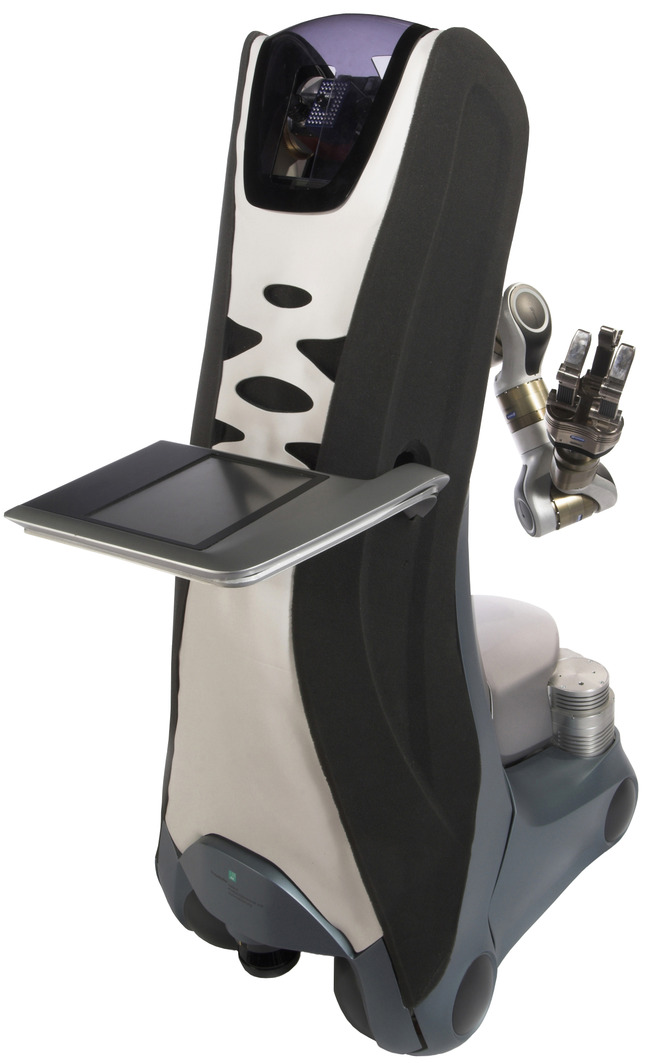
\includegraphics[width=3cm]{./image/Care_o_bot_3.jpg}
   		\end{column}
	\end{columns}
\end{frame}

\begin{frame}
	\frametitle{Où le trouve t-on?}
	\begin{itemize}
	\item Type :
		\begin{itemize}
		\item Intérieur
		\item Connu
		\end{itemize}
	\item Exemple :
		\begin{itemize}
		\item Environement domestique
		\item Maison de retraitre 
		\end{itemize}
	\end{itemize}
\end{frame}


\begin{frame}
	\frametitle{De quoi est-il composé?}
	\begin{columns}[T]
		\begin{column}{.5\textwidth}
			\begin{itemize}
			\item Caractéristiques:
				\begin{itemize}
				\item un bras à 7 degrés de liberté
				\item 8 moteurs contrôlant 4 roues
				\item un système de vision composé de
                                  2 caméra et un d'aun capteur de
                                  profondeur
				\end{itemize}
			\end{itemize}
		\end{column}
   		\begin{column}{.5\textwidth}
			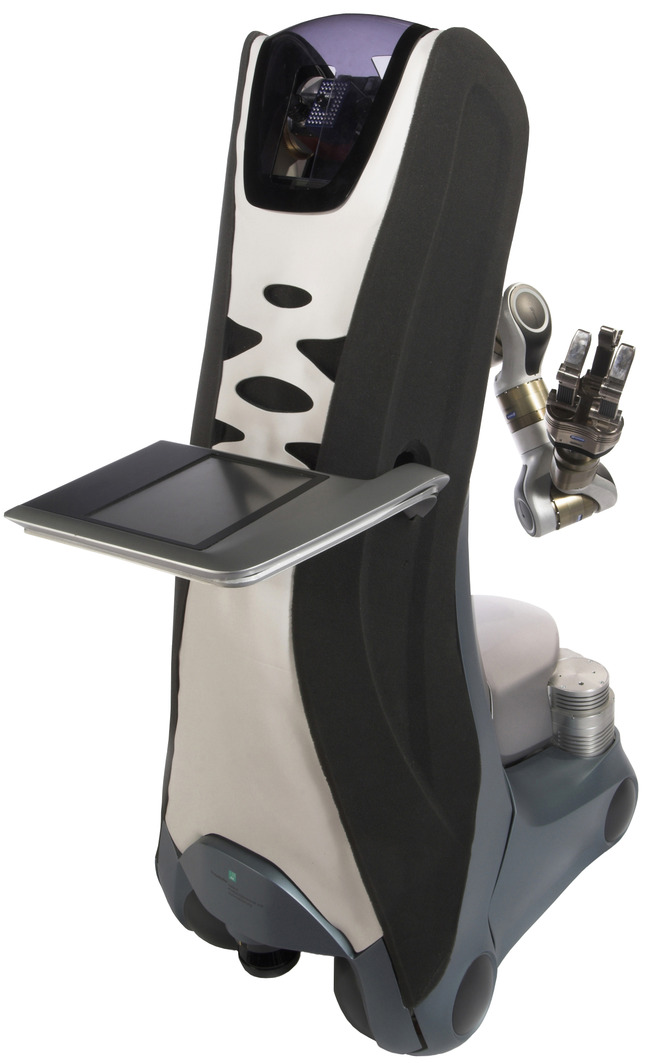
\includegraphics[width=3cm]{./image/Care_o_bot_3.jpg}
   		\end{column}
	\end{columns}
\end{frame}

\subsection{Applications}
\begin{frame}
	\frametitle{Transport d'objet}
	\begin{center}
	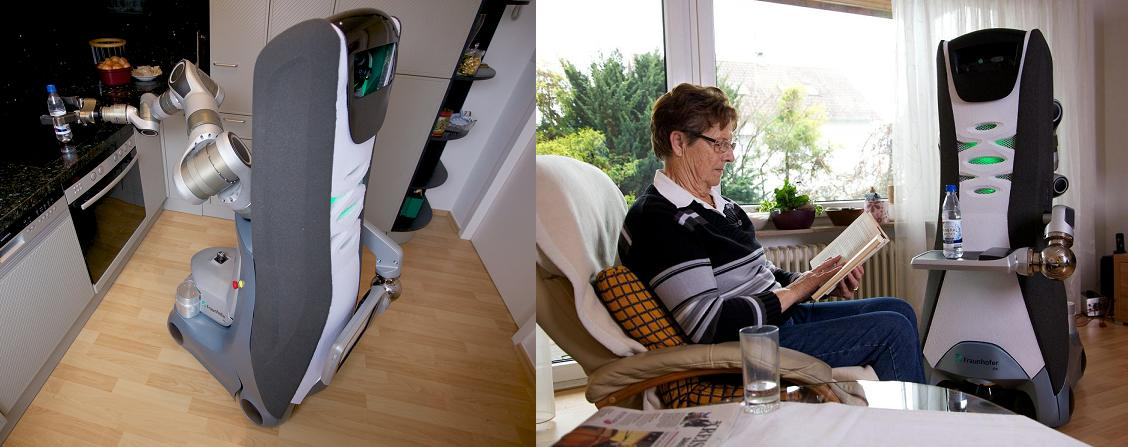
\includegraphics[scale = 0.36]{./image/Fetch_and_Carry2.JPG}
	\end{center}
\end{frame}

\begin{frame}
	\frametitle{Divertissement et communication}
	\begin{center}
	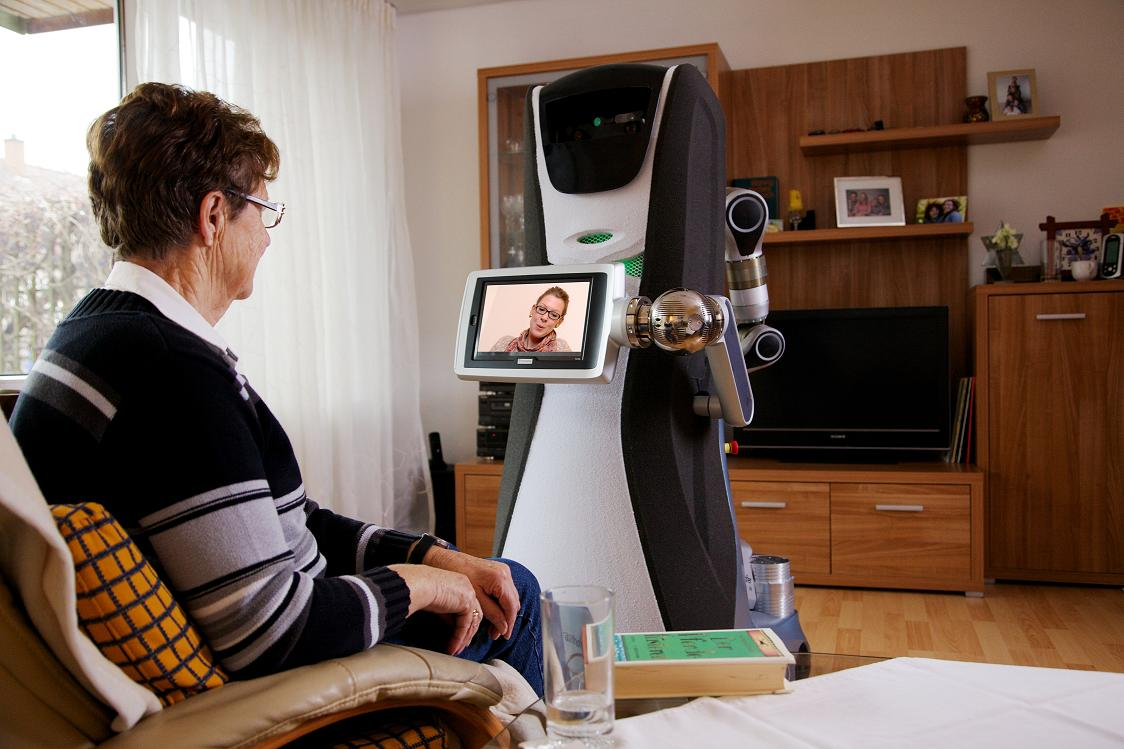
\includegraphics[scale = 0.30]{./image/Communication.JPG}
	\end{center}
\end{frame}

\begin{frame}
	\frametitle{Situation d'urgence}
	\begin{center}
	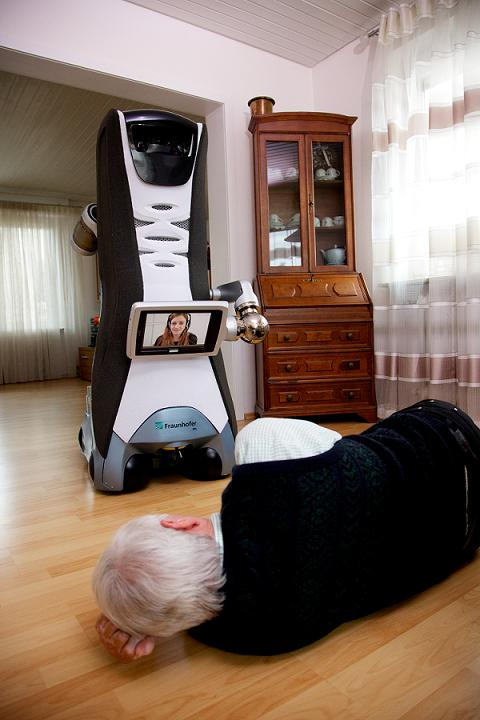
\includegraphics[scale = 0.36]{./image/EmergencySupport.JPG}
	\end{center}
\end{frame}

